%version of 01-21-20

\chapter{Solutions/Hints for selected exercises}
\label{ch:Exercises}



\section*{Exercises: Chapter 2}

\begin{itemize}
\item
{\bf 2.2. Meeting people at a party}

{\em Some two attendees shake the same number of hands.}
\medskip

%
This observation follows from the \textit{pigeonhole principle}:
If $n+1$ pigeons occupy $n$ pigeonholes, then some hole contains
at least $2$ pigeons.
\smallskip

This principle guarantees that some two attendees shake the same
number of hands.  To wit, the number of people that each attendee {\em
  does not know} belongs to the set $\{ 0, 1, \ldots, 2n-2 \}$,
because each person knows him/herself and his/her partner.  Since
there are $2n$ handshakers (the pigeons) and $2n-1$ numbers of hands
to shake (the boxes), some two shakers must shake the same numbers of
hands. 
\medskip
\item
{\bf 2.4. Bi-colored necklaces in tubes}

You have a {\it necklace} composed of $2n$ jewels: $2a$ black jewels and $2b$ white jewels.  For illustration, the necklace in Fig.~\ref{fig:sample-necklace} has $n = 6$, $a = 5$, and $b =1$.
\begin{figure}[ht]
\begin{center}
       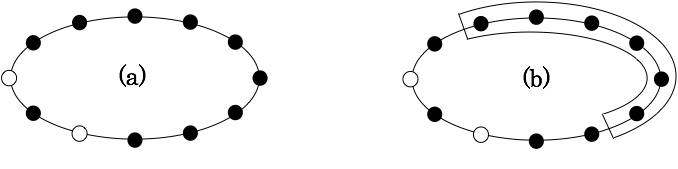
\includegraphics[scale=0.35]{FiguresMaths/SampleNecklace}
\caption{(a) A necklace having $12$ jewels: $10$ black and $2$ white.  (b) The necklace in a tube.}
\label{fig:sample-necklace}
\end{center}
\end{figure}

In part (a) of the figure, the necklace is unadorned; in part (b), the necklace appears within a length-$n$ {\it tube} which isolates one string---i.e., half-necklace---of $n$ jewels from the complementary string.

\smallskip

\begin{prop}
For any bi-colored necklace of the form described---i.e., with even numbers of jewels, black jewels, and white jewels---there is a way to position the tube so that inside the tube and outside the tube, there are equally many jewels, equally many black jewels, and equally many white jewels.
\end{prop} 

\smallskip

Slide the tube around the necklace, and count both black and white jewels at each step.  
How can these numbers change in a single step?
\medskip

\item
{\bf 2.6. Using {\em geometric} intuition to sum inverse powers of $4$}

{\sc Lesson:} Exploiting geometric intuition toward a sophisticated end.

\smallskip

We turn to a variant of Proposition~\ref{thm:sumof-1/4-induction}.  This time, we focus on the entire infinite summation
\[ S \ \ = \ \  {1 \over 4} \ + \  {1 \over 4^2} \ + \cdots + \ {1 \over 4^k} \ + \cdots  \]
and we do so from a geometric point of view.

\smallskip

We prove in Proposition~\ref{thm:sum-finite-geometric-series}(b) that this infinite summation converges to the value ${1 \over 3}$.  A simple way to see this is to multiply the summation $S$ term by term by the fraction $1/4$.  We observe---just by inspection---that the resulting product, which clearly has the value $S/4$, equals $S - 1/4$, so that $S = 1/3$.

\smallskip

We have now described the process at a very high level.  
Your assignment is to flesh out the details.  {\em Prove that the four sub-triangles
\begin{itemize}
\item
are similar to one another
\item
are similar to the original triangle
\item
have area which is $1/4$ that of the original triangle
\end{itemize}
Assemble these facts into an evaluation of the sum $S$.
}

\noindent \textit{Solution.}
A rapid analysis of the small values of $k$ leads to the guess $(\frac{1}{4})^k = \frac{1}{3}$.
 
The solution is depicted in Fig.~\ref{Fig:Sumgeo1sur4}. 
\begin{figure}
\begin{center}
        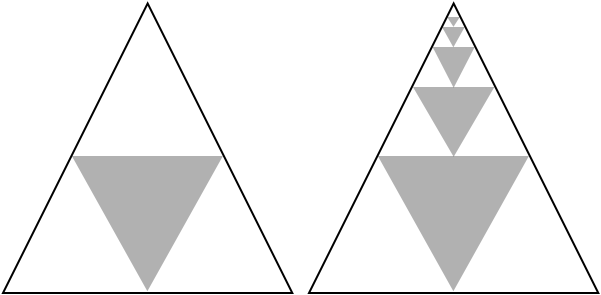
\includegraphics[scale=0.3]{FiguresArithmetic/SumGeometric1sur4}
        \caption{Graphical construction. Assuming the total area is 1, the area of the grey internal triangle (left) is $\frac{1}{4}$.
        As the grey area is one third at each layer (right), the whole area is $\frac{1}{3}$.
        By the double counting Fubini's principle, this area is the sum of the $\frac{1}{4^k}$ (for $k \geq 1$).}
        \label{Fig:Sumgeo1sur4}
\end{center}
\end{figure}

Finding such a triangular pattern may not be considered as an easy task.
However, as stated in the problem, the main point is to divide an elementary surface
into four equal pieces. 
Squares (or even worse disks) are not simple to use in this context while isosceles triangles 
are a \textit{natural} structure. 

\end{itemize}

\ignore{*************************
\subsection{A graphical proof}

\noindent \textit{The problem.}
%\label{thm:an-arithmetic-identity}
Prove the following property:

or any positive integer $n$,
\[ \Delta_{2n-1} \ = \ n + 4 \Delta_{n-1}. \]
\medskip

\noindent \textit{The solution.}

Consider the arithmetic series in (\ref{eq:arith-seq}) for the case
$a=1$ and $b=4$.  
By Proposition~\ref{thm:sum-of-arithmetic-series},
this series, call it $S^{(1,4)}(n)$, has the sum
\begin{equation}
\label{eq:triangles}
S^{(1,4)}(n) \ = \ n + 4 \Delta_{n-1}.
\end{equation}

Let us represent the sum $\Delta_{n-1}$ in the natural way as a
triangle of tokens.  This triangle has a base of $n-1$ tokens, upon
which sits a row of $n-2$ tokens, upon which sits a row of $n-3$
tokens, \ldots, all the way to the apex, which has a single token.

Now, let us view equation (\ref{eq:triangles}) as giving us access to four
copies of the preceding triangle of tokens.  Let us arrange these
triangles in the manner depicted in Fig.~\ref{fig:Delta(n)4}.
\begin{figure}[ht]
\begin{center}
       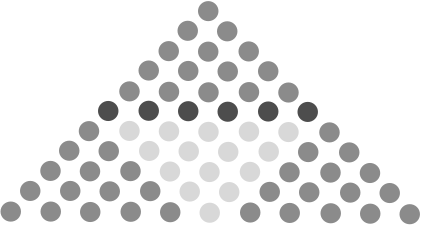
\includegraphics[scale=0.5]{FiguresMaths/Delta4}
 \caption{Arranging the four triangles plus a row to obtain a new (bigger) triangle.}
       \label{fig:Delta(n)4}
\end{center}
\end{figure}
Now, ``complete the picture'' by adding an ``extra'' row of $n$
tokens at row $n$ of the figure (these are depicted in dark gray in
the figure).  The four small triangles, augmented by the ``extra'' row
of $n$ tokens has clearly become a representation  of $\Delta_{2n-1}$
by tokens.

We now have a purely pictorial proof of the proposition. 

*************************}


%%%%%%%%%%%%%%%%%%%%%%%%%%%%%%%%%%%%%%%%%%%%%%


\section*{Exercises of Chapter 3}

\begin{itemize}
\item
{\bf 3.8. More connections between strings and functions}
\medskip

{\em Craft an argument that predicts the number of permutations, based on the size of set $S$.}
\smallskip

{\em Hint:}
\begin{itemize}
\item
As you create a new string of numbers, in how many ways can you choose {\em the first number}? 
{\em the second number}? \ldots
\item
Based on your answers for the first and second and third numbers of the new string, 
in how many ways can you choose {\em the first two numbers---i.e., the first {\em pair} of numbers}? 
{\em the next two numbers}? \ldots
\end{itemize}
  \item
{\em Strengthen your argument by listing all permutations of  $S' =  \{1,2,3,4,5\}$.}

\smallskip

Write small---there are a lot of permutations.
  \item
{\em Extrapolate from your argument to determine the number of permutations of the set 
$S" =  \{1,2,3, \ldots, n\}$, as a function of $n$.}

\end{itemize}


%%%%%%%%%%%%%%%%%%%%%%%%%%%%%%%%%%%%%%%%%%%%%%%%
\section*{Exercises: Chapter 4}

\begin{itemize}
\item
{\bf 4.5. The rationals ($\Q$) and the integers ($\N$) are equinumerous}
\smallskip

{\em Provide a {\em detailed} proof of Proposition~\ref{thm:|Q|=|N|}.}  
Informally, there are equally many integers as there are rationals.

\end{itemize}



\ignore{***************************************
\subsection{Complex
  multiplication via $3$ real multiplications}
\index{complex number!multiplication via 3 real multiplications}

\noindent {\it The problem.}
%\label{thm:complex-mult-3real}
Show how to compute the product of two complex numbers using only {\em three}
real multiplications rather than four.
\medskip

\noindent {\it The solution.}
Although implementing (\ref{eq:complex-mult}) ``directly'' correctly
produces the product $\kappa = (a+bi) \cdot (c+di)$, there is another
implementation that is {\em more efficient}.  Specifically, the
following recipe computes $\kappa$ using only {\em three} real
multiplications instead of the four real multiplications of the
``direct'' implementation.  We begin to search for this recipe by
noting that our immediate goal is to compute both Re$(\kappa) = ac-bd$
and Im$(\kappa) = ad+bc$.  We can accomplish this by computing the
{\em three} real products
\begin{equation}
\label{eq:complex-mult-3a}
(a+b) \cdot (c+d); \ \ \ \ \
ac;  \ \ \ \ \ bd
\end{equation}
and then noting that
\begin{equation}
\label{eq:complex-mult-3b}
\begin{array}{lcl}
\mbox{Im}(\kappa) & = & (a+b) \cdot (c+d) - ac -bd, \\
\mbox{Re}(\kappa) & = & ac -bd
\end{array}
\end{equation}
We thereby achieve the result of the complex multiplication described
in (\ref{eq:complex-mult}) while using only {\em three} real
multiplications.


%%%
\subsection{Another proof for irrationality of $\sqrt{2}$}


\noindent \textit{The problem.}
Prove the irrationality of $\sqrt{2}$ using a geometrical argument.
\medskip

\noindent \textit{Hint.}
The proof is by contradiction. 

Consider $\sqrt{2}$ is rational, which means there exists a pair of integers $(a,b)$
such that $\sqrt{2} = \frac{a}{b}$ (where $a$ is larger than $b$).
Among all possible pairs, take the unique irreductible ratio.

Represent this expression geometrically by the corresponding isosceles triangle
which is the one of minimal surface. 

The contradiction comes by constructing another isosceles triangle with a smaller surface.
%Squaring this expression leads to $2.b^2 = a^2$.
\medskip

\noindent \textit{The solution.}

The solution is depicted in Fig.~\ref{Fig:sqrtbisInit} and~\ref{Fig:sqrtbisFin} . 
\begin{figure}
\begin{center}
        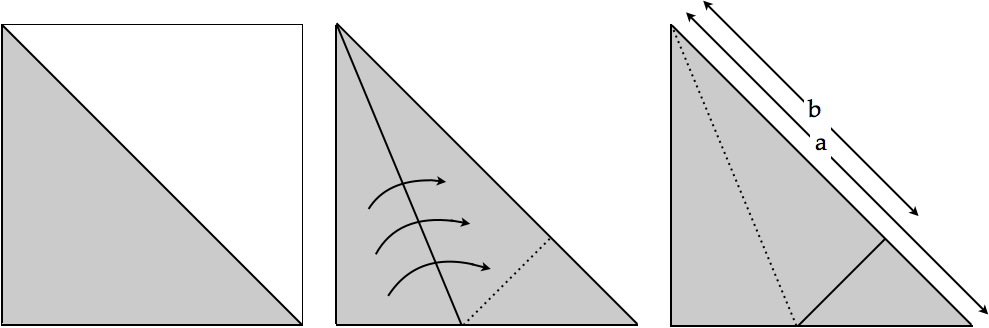
\includegraphics[scale=0.3]{FiguresArithmetic/sqrtbisInit}
        \caption{First step: folding the triangle along the side.}
        \label{Fig:sqrtbisInit}
\end{center}
\end{figure}
\begin{figure}
\begin{center}
        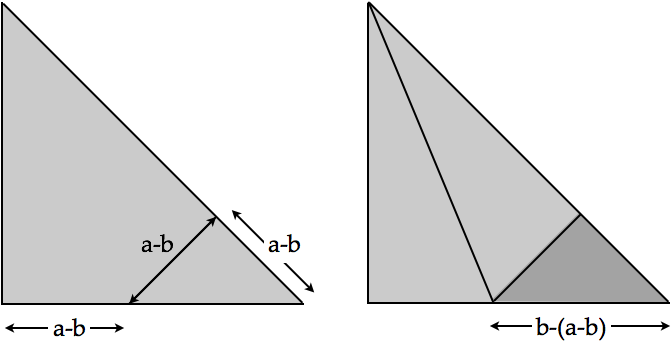
\includegraphics[scale=0.3]{FiguresArithmetic/sqrtbisFin}
        \caption{Second step. The sides of the small isosceles triangle are integers.}
        \label{Fig:sqrtbisFin}
\end{center}
\end{figure}
****************************}


%%%%%%%%%%%%%%%%%%%%%%%%%%%%%%%%

\ignore{*******************************
\section{Chapter 5}


\subsection{A ``trick'' for squaring certain integers}


\noindent \textit{The problem:}

Let $n$ be any number that has a $2$-digit decimal numeral of the form

\hspace{.25in}$5.\delta$ \ \ \ \ $(\delta \in \{ 0,1,2,3,4,5,6,7,8,9\})$.

\noindent
Then the square of $n$ is the integer

\hspace{.25in}$25 \ + \ \delta \cdot (\delta +1)$
\medskip

\noindent \textit{The solution:}

We can rewrite the premise of the proposition in the form
\[ n \ = \ 10 \cdot \delta + 5 \]
It is now easy to invoke Proposition~\ref{prop:(a+b)(c+d)} and the
distributive law to compute that

\[ n^2 \ = \ 100 \cdot \delta \cdot (\delta+1) + 25 \]
To wit: 
\[
\begin{array}{lclll}
n^2 & = & (10 \cdot \delta + 5)^2 & & \mbox{Given} \\
    & = & 100 \cdot \delta^2 \ + \ 100 \cdot \delta \ + \ 25
              & & \mbox{the proposition} \\
    & = & 100 \cdot (\delta^2 \ + \ \delta) \ + \ 25
              & & \mbox{factoring: distributive law} \\
    & = & 100 \cdot \delta \cdot (\delta + 1) \ + \ 25
              & & \mbox{factoring: distributive law} \\
\end{array}
\]
A parlor trick has become a mathematical demonstration!


%%%
\subsection{Revisiting a very old problem}

\noindent \textit{The problem:}

This problem comes from babylonians in the 18th century BC.
The numeral system was in base 60, and the problem was to determine the length of the side of a square which was part of a larger rectangle.
The following figure details the process.
\medskip

\noindent \textit{The solution:}

The idea of the proof is to represent the left hand side by the square $x^2$ beside a rectangle $60 \times x$
(see Fig.~\ref{fig:equationBabillon}).
Recall that the coefficient of $x$ in the equation is $1$, this corresponds to $60$ in the considered basis. 
Then, split the right rectangle into two equal parts and move one part a the bottom of the left square.
The final figure shows the whole square whose surface is equal to $45$ plus the surface of the white square
whose surface is equal to $30 \times 30$.
In base $60$, this is equal to $15$. 
$45+15 = 60$, thus, the big square is the unit square, its side is $60$.
Thus, the length of the initial square is equal to $60-30=30$.
\begin{figure}[htb]
\begin{center}
       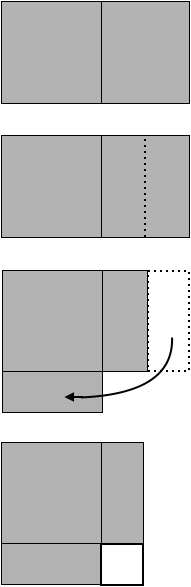
\includegraphics[scale=0.4]{FiguresArithmetic/tabletteMesopotamie}
\caption{Solving $x^2 + x = 45$.}
\label{fig:equationBabillon}
\end{center}
\end{figure}
*****************************}


%%%%%%%%%%%%%%%%%%%%%%%%%%%%%%%%%%%%%%%%%%

\section*{Exercises: Chapter 6}

\begin{itemize}
\item
{\bf 6.4. Evaluating $S_1(n) = \sum_{i=1}^n \ i$, using the fact that $S_2(n) = \sum_{i=1}^n \ i^2$}

Say that someone gives you a machine that can compute the summation of the first $n$ perfect squares, given $n$ as an input:
\[ S_2(n)  \ = \ 1 \  + \ 4 \ + \ 9 \ +  \cdots + \ n^2 \]

{\em Show how to use this machine in order to compute the sum of the first $n$ integers.}

\medskip
The idea here is to write the sum by extracting the first and the last element
of the sum of squares.
\medskip

$S_{n+1} = 1 + \sum_{i=1}^{n+1} i^2$

$S_{n+1} = (\sum_{i=1}^{n} i^2) + (n+1)^2$

where $\sum_{i=1}^{n+1} i^2 
= \sum_{i=0}^{n} (i-1)^2 
= \sum_{i=0}^{n} (i^2-2i+1) 
= \sum_{i=0}^{n} i^2- 2 ( \sum_{i=0}^{n} i) + (n+1)
= \sum_{i=1}^{n} i^2- 2 ( \sum_{i=1}^{n} i) + (n+1)$

Thus, 
$\sum_{i=1}^{n} i^2- 2 ( \sum_{i=1}^{n} i) + (n+1) = (\sum_{i=1}^{n} i^2) + (n+1)^2$

$-2 \Delta_n + (n+1) =  (n+1)^2$

$\Delta_n =  (n+1)^2-(n+1) = n(n+1)$
\medskip

\item
{\bf 6.6. Evaluating a geometric summation pictorially}

In Section~\ref{sec:summing-geometric-series:techniques}, we used Thales's theorem about similarity in triangles (Theorem~\ref{thm:Thm-of-Thales-similarity}) to sum the simple infinite geometric series $\sum_{i=0}^\infty \ b^i$.  It turns out that a modest modification of that evaluation strategy allows us also to evaluate the truncated versions of that series, namely, the summations
\[ S^{(b)}(n) \ = \ \sum_{i=0}^n \ b^i \]

{\em Use the following figure to evaluate $S^{(b)}(n)$.}

\centerline{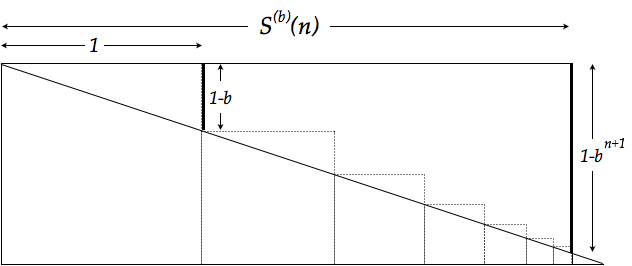
\includegraphics[scale=0.4]{FiguresArithmetic/ThalesGeometricSumFiniteSol}}
\medskip

\item
{\bf 6.7. A direct proof that the harmonic series diverges}

{\em Develop a proof of the divergence of the harmonic series 
\[ S^{(H)} \ = \ \sum_{k=1}^\infty \ {1 \over k} \]
\begin{itemize}
\item
partitioning $S^{(H)}$'s terms into groups whose sizes are successive powers of $2$
\item
developing an argument based on the sums within the groups.
\end{itemize}
}

\smallskip

{\em For clarification:}
The partitioning step operates as follows:
{\footnotesize
\[ 
\begin{array}{ll}
S^{(H)} 
             & = \ 1 \ + \ {1 \over 2} + {1 \over 3} + {1 \over 4} + {1 \over 5} + {1 \over 6}+ {1 \over 7} + {1 \over 8} + {1 \over 9} + {1 \over 10}+ {1 \over 11}  +{1 \over 12} + {1 \over 13} + {1 \over 14}+ {1 \over 15} + \cdots \\
             & \\
  & = \ (1)  +  \left( {1 \over 2} + {1 \over 3} \right)  +  \left( {1 \over 4} + {1 \over 5} + {1 \over 6}+ {1 \over 7} \right)  +  \left( {1 \over 8} + {1 \over 9} + {1 \over 10}+ {1 \over 11}  +{1 \over 12} + {1 \over 13} + {1 \over 14}+ {1 \over 15} \right) \ +\cdots
\end{array} \]
}


A first solution is to group the terms according to powers of $2$. 
Then, the sum within each group is between $\frac{1}{2}$ and $1$, thus,
$H_n > \frac{1}{2}.n$
\medskip

{\em Propose another more precise analysis by gathering the terms 3 by 3}

$S_k = (\frac{1}{3k-1} + \frac{1}{3k} + \frac{1}{3k+1} )$ for $k\geq1$, 

$H = 1 + S_1 + ... + S_k + ... > 1 + 3.\frac{1}{3} + 3.\frac{1}{6} + ... + 3.\frac{1}{3k} + ... $

since $S_k > 3.\frac{1}{k} $.

The proof is by contradiction:

if $H$ is finite, from the previous relation we have: $H > 1 + H$, which is obviously impossible.
\medskip

Moreover, the first way of  bounding the sum tells us about its value (actually, we know the value at a factor of $2$):

$\frac{log(n)+1}{2} < H_n < log(n)+1$. Thus, $H_n = O(log(n))$
\medskip

\item
$\oplus$ {\bf 6.8. Summations, and summations of summations}

{\sc Lesson:} Practice manipulating summations; gain familiarity with basic sums

\smallskip

By definition:
\[ Id_n \ \eqdef \ \sum_{k=1}^n \ 1 \ = \ 1 + 1 + \cdots +1 \  = \ n \]

We have proved in multiple ways:
\[ \Delta_n \ \eqdef \  \sum_{k=1}^n \ k \ = \ 1+2+3+ \cdots +n \ = \ \frac{1}{2} Id_n \cdot (n+1) \]

\smallskip

This exercise picks up where these two examples leave off.

  \begin{enumerate}
  \item 
{\em Prove that}\footnote{The sum of the the first $n$ triangular numbers, $\sum_{k=1}^n \ \Delta_k$, is often denoted $\Theta_n$.  We employ instead the nonstandard name $\widehat{T}_n$ to ensure that we do not confuse the newcomer who has recently learned about the role of the letter $\Theta$ in asymptotic notation.} 
\[ \widehat{T}_n \ \eqdef \  \sum_{k=1}^n \ \Delta_k \ = \   
\Delta_1 + \Delta_2 + \cdots + \Delta_n \ = \ \frac{1}{3} \Delta_n \cdot (n+2) \]

  \item
$\oplus \oplus$
{\em Develop and verify a formula for the summation:}
\[ \Upsilon_n  \ \eqdef \  \sum_{k=1}^n \ \widehat{T}_k \ = \  
\widehat{T}_1 + \widehat{T}_2 + \cdots + \widehat{T}_n \]

  \item
{\em Prove the following identities involving $\Delta_n$.  For all $n \in \N^+$:}
    \begin{enumerate}
    \item
$\Delta_n \ + \ \Delta_{n-1} \ = \ n^2$

\smallskip

This is a straightforward exercise in algebraic manipulation.  Can you {\em also} find an ``interesting" proof of this identity, say one that employs a ``pictorial" representation of $\Delta_n$?

 \item
$\Delta_n^2 \ - \ \Delta_{n-1}^2 \ = \ n^3$

\smallskip

{\em Hint}: Try ``playing" with simple manipulations of the equation 
\[ \Delta_n \ = \ n \ + \ \Delta_{n-1} \]
which defines $\Delta_n$.
   \end{enumerate}

  \item
$\oplus$
{\em Derive a closed-form expression for the sum}
\[ \widehat{T}_n \ + \ \widehat{T} _{n-1} \]

\smallskip

{\em Hint}: Recall that the sums $\widehat{T}_i$ are defined as sums of $\Delta_j$, which, in turn, are defined by closed-form expressions.  Lots to ``play" with!
\end{enumerate}
\end{itemize} 


\ignore{*****************************
%%%
\subsection{Sum of perfect cubes}

\noindent \textit{The problem.}
Show that the sum of $n$ first cubes is equal to a perfect square, and more precisely, $\Delta_n^2$.
\medskip

\noindent \textit{The solution.}
The proof is based on an hold and simple pattern that we learned in elementary school.
\medskip

\index{$n^2$ as sum of first $n$ odd integers!a proof from elementary school}

%
Consider the following reasoning which emerges from the way
multiplication tables are developed in elementary school.  
Let us first illustrate the idea using the case $n=5$.
\begin{equation}
\label{eq:Fubini-table}
\begin{array}{rrrrr}
1  &  2 &  3 &  4 &  5 \\
2  &  4 &  6 &  8 & 10 \\
3  &  6 &  9 & 12 & 15 \\
4  &  8 & 12 & 16 & 20 \\
5  & 10 & 15 & 20 & 25 \\
\end{array}
\end{equation}
Write the integers $1, 2, \ldots, n$ in a row.  Below this row, write
the doubles of these integers.  Below the ``double'' row, write the
triples of the integers.  Below the ``triple'' row, write the
quadruples of the integers, then the quintuples, and so on.  Note that
the resulting table is {\em symmetric:} its rows are identical to its
columns.
\medskip

Using again Fubini's rearrangement stratagem, we now count all the integers in
the table in two different ways.
\begin{enumerate}
\item
We sum the entries of our table by peeling away successively larger
reversed instances of the letter ``$L$'' (as in our earlier
``pictorial'' proof of
Proposition~\ref{thm:squares-odd-integers-Gauss}).  We find that the
integers in each ``$L$'' sum to a perfect cube.
Actually, the diagonal is (by definition) equals to the square.
\[
\begin{array}{rrrrrrrrr|rrc}
1  &    &    &    &    &   &     &    &   & 1   & = 1^3 \\
2  &  4 &  2 &    &    &   &     &    &   & 8   & = 2^3 \\
3  &  6 &  9 &  6 &  3 &   &     &    &   & 27  & = 3^3 \\
4  &  8 & 12 & 16 & 12 &  8 &  4 &    &   & 64  & = 4^3 \\
5  & 10 & 15 & 20 & 25 & 20 & 15 & 10 & 5 & 125 & = 5^3
\end{array}
\]

\item
We sum the successive rows of the $n \times n$ table (\ref{eq:Fubini-table}).  
The first row of the table sums to $\Delta_n$; the second row sums to $2
\Delta_n$; the third row sums to $3 \Delta_n$; \ldots; the last row sums
to $n \Delta_n$.  
Thus, the aggregate sum of the table's rows is 
\[ (1 + 2 + \cdots + n) \cdot \Delta_n \ = \ \left(\Delta_n \right)^2 \]
\end{enumerate}
We conclude that
\[
\sum_{i=1}^n i^3 \ = \  \left(\Delta_n \right)^2
\]
************************************************}


%%%%%%%%%%%%%%%%%%%%%%%%%%%%%%%%%%%%%

\section*{Exercises: Chapter 7}


\ignore{****************************
\subsection{Handling asymptotic}


\noindent \textit{The problem.}

Prove that $f = O(g)$ and $h = O(k)$ for functions $f,g,h,k$ implies that
$f+h = O(g+k)$


\subsection{What's wrong?}

\noindent \textit{The aim.}
to investigate a proof which leads to surprising results.


\begin{enumerate}
\item
Let consider the infinite sum $A = 1-1+1-1+ \ldots$

show that $A=\frac{1}{2}$ (hint: compute $1-A$)
\item
Let now consider the other infinite sum $B=2-3+4-5+6 \ldots$

show that $B=\frac{1}{4}$ (hint: compute $A+B-1$)
\item 
Compute the sum of the integers $C=1+2+3+4+ \ldots$

show that $C=-\frac{1}{12}$ (hint: compute $C-B=4+8+12+16+ \ldots$)
\end{enumerate}

\medskip

\noindent \textit{The problem.}

What's wrong?

\medskip

\noindent \textit{The solution.}
First, summing up positive number should be positive, 
and second, the sum of the integers should be infinite...

Then, how to analyze the previous result/proof?
******************************************************}




%%%%%%%%%%%%%%%%%%%%%%%%%%%%%%%%%%


\section*{Exercises: Chapter 8}

\begin{itemize}

\item
{\bf 8.2. Discovering fractal-like structure in Pascal's triangle}

Modular arithmetic can do wondrous, unexpected things with regular structures.  If one takes a system whose structure is governed by arithmetic and substitutes {\em modular} arithmetic for ordinary arithmetic, then the system's structure is somehow going to be ``folded into itself".  We illustrate this fact within a rather complex framework in Appendix~\ref{Appendix:tree-DB}; the ``folded" structures there are trees.  We illustrate the fact within a rather elementary framework in this exercise; the ``folded" structures here arise from Pascal's triangle.

\medskip

Take Pascal's triangle, choose a positive integer $m$, and replace each of the triangle's entries---which are, of course, the binomial coefficients---by that entry modulo $m$.  As illustrated in Fig.~\ref{fig:TriangleModulo5},
%Figs.~\ref{fig:TriangleModulo5raw} and~\ref{fig:TriangleModulo5shade}.
\begin{figure}[ht]
\begin{center}
	\includegraphics[scale=0.18]{FiguresArithmetic/TrianglePascalModulo5init.png}
	\hspace*{.1in}
	\includegraphics[scale=0.18]{FiguresArithmetic/TrianglePascalModulo5.png}
	        \caption{Pascal's triangle modulo $5$: (left) the ``raw" version; (right)
	        with the reproducible pattern highlighted.}
        \label{fig:TriangleModulo5}
\end{center}
\end{figure}
a wondrous transformation happens.  The first $m$ levels of the triangle get replicated endlessly, with an inverted $(m-1)$-level triangle whose entries are all $0$.  (In the figure, the inverted triangle of $0$s is depicted in gray.) 
The original triangle has been transformed into a fractal-like repetitive structure whose pattern of repetitions is dictated by the parameter $m$.

\medskip

{\em Prove that the described transformation occurs.}

%
\medskip\item
{\bf 8.4. Divisibility among integers: via the Fundamental Theorem of Arithmetic}

  \begin{itemize}
\item
b. {\bf The sieve of Eratosthenes and its implications}

We formulate the sieve as a regimen for labeling integers with their prime factors.  For simplicity, we use the label $\lambda_p$ to identify integers which are multiples of prime $p$.

\medskip

We begin with the linear array of positive integers:

$\begin{array}{c|c|c|c|c|c|c|c|c|c|c|c|c}
1 & 2 & 3 & 4 & 5 & 6 & 7 & 8 & 9 & 10 & 11 & 12 & 13
\end{array}$ \ldots

\medskip

We label the multiples of $2$ (i.e., the even numbers):

$\begin{array}{c|c|c|c|c|c|c|c|c|c|c|c|c}
1 & 2 & 3 & 4 & 5 & 6 & 7 & 8 & 9 & 10 & 11 & 12 & 13 \\
 & \lambda_2 & & \lambda_2 & & \lambda_2 & & \lambda_2 & & \lambda_2 & & \lambda_2 &
\end{array}$ \ldots

\medskip

We label the multiples of $3$:

$\begin{array}{c|c|c|c|c|c|c|c|c|c|c|c|c}
1 & 2 & 3 & 4 & 5 & 6 & 7 & 8 & 9 & 10 & 11 & 12 & 13 \\
 & \lambda_2 & & \lambda_2 & & \lambda_2 & & \lambda_2 & & \lambda_2 & & \lambda_2 & \\
 & & \lambda_3 & &  & \lambda_3 & & & \lambda_3 & & & \lambda_3 &
\end{array}$ \ldots

\medskip

We label the multiples of $5$:

$\begin{array}{c|c|c|c|c|c|c|c|c|c|c|c|c}
1 & 2 & 3 & 4 & 5 & 6 & 7 & 8 & 9 & 10 & 11 & 12 & 13 \\
 & \lambda_2 & & \lambda_2 & & \lambda_2 & & \lambda_2 & & \lambda_2 & & \lambda_2 & \\
 & & \lambda_3 & &  & \lambda_3 & & & \lambda_3 & & & \lambda_3 & \\
 & & & & \lambda_5 & & & & & \lambda_5 & & & 
\end{array}$ \ldots

\bigskip

The sieve affords one a wonderful perspective for perceiving the patterns that drive mathematical insights.  Here are a few results for you to prove, which are suggested by a perusal of the sieve.

\smallskip

{\em Prove the following results.}
     \begin{enumerate}
     \item
\begin{prop}
Every integer $n>1$ is divisible by at least one prime number.
\end{prop}

     \medskip\item
\begin{prop}
Every sequence $k+1, \ldots, k+p$ of $p$ integers contains a multiple of $p$.
\end{prop}

      \medskip\item This result calls for ``second-order" insights from the sieve.
\begin{prop}
Every product of four consecutive integers, $(k+1) \cdot (k+2) \cdot (k+3) \cdot (k+4)$ is divisible by $4!$
\end{prop}

\smallskip

{\em Hint}:  Look at the {\em multiplicity} with which a given prime divides a given number, particularly within the context of the spacings of the divisibilities---e.g., every even number that is $2 \times$ an odd number is followed by an even number that is $2 \times$ an even number.  

\smallskip

{\em Extend this exercise to divisors other than $4$.}

\medskip\item
The sieve affords us an alternative proof that there are infinitely many primes, particularly via the alternative version that is due to Leonhard Euler.  In this version of the sieve, each prime and all of its multiples are removed from the sieve as soon as their existence is acknowledged.  Our earlier construction of Eratosthenes's version of the sieve now becomes:

\medskip

$\begin{array}{|l||c|c|c|c|c|c|c|c|c|c|c|c|c|c|}
\hline
\mbox{Initial array:} &
1 & 2 & 3 & 4 & 5 & 6 & 7 & 8 & 9 & 10 & 11 & 12 & 13 & \cdots \\
\mbox{after prime $2$ is processed:} &
1 &  & 3 &  & 5 &  & 7 &  & 9 &  & 11 &  & 13 & \cdots \\
\mbox{after primes $2, 3$ are processed:} &
1 &  &  &  & 5 &  & 7 &  &  &  & 11 &  & 13 & \cdots \\
\mbox{after primes $2, 3, 5$ are processed:} &
1 &  &  &  &  &  & 7 &  &  &  & 11 &  & 13 & \cdots \\
\hspace*{.8in} \vdots  &
 &  &  &  &  &  & \vdots &  &  &  &  &  &  & \\
\hline
\end{array}$

\bigskip

{\em Use Euler's sieve to prove that there are infinitely many primes.}

\medskip

{\em Hint:} If there were only finitely many primes, then at some (finite) stage in processing the sieve, the list of integers would be reduced to the single integer $1$.
\end{enumerate}
\end{itemize}


 \medskip\item

{\bf 8.5. The ``density"  of divisible pairs of numbers}

{\em Prove that the following assertion is true for every positive integer $n$.}

\begin{prop}
For every positive integer $n$:  If you remove {\em any} $n+1$ integers from the set $S = \{ 1, 2, \ldots, 2n\}$, then the set of removed integers contains at least one pair $p$ and $q > p$ such that $p$ divides $q$.
\end{prop}


\smallskip

Let $\alpha_i$ be the elements of this set of $n+1$ elements.
Write $\alpha_i = 2^k \times m$ where $m$ is odd (and $k \geq 0$).

The $2n$ numbers of the sequence are decomposed into multiples of powers of $2$.
When there are multiple ways, we take the one with the largest power of $2$ in order to make the decomposition unique.
Example for $n=7$:

1, 3, 5, 7, 9, 11, 13

2, 6, 10, 14

4, 12

8
\medskip


%The sketch of the proof is as follows.
\begin{enumerate}
\item
 $\alpha_i = 2^k \times m$ 
 
$m$ belongs to the $n$ numbers $\{1,3,5, \ldots, 2n-1 \}$

As we are considering $n+1$ integers, from the pigeon hole principle, there are two numbers with the same value of $m$. 
\item 
Thus, $2^{k1} \times m$ and $2^{k2} \times m$

$p$ is the smallest one, which divides $q$ (the largest one).
\end{enumerate}


\medskip\item

{\bf 8.8. The set $\Q$ of rational numbers is countable}

{\em Prove Proposition~\ref{thm:|Q|=|N|}: $|\Q| \ = \ |\N|$}

\smallskip

{\em Hint}.  Begin by reviewing Proposition~\ref{thm:|NxN|=|N|}, which asserts the technically simpler proposition: $|\N \times \N| \ = \ |\N|$.  What is the relevance of that result to this problem?

\end{itemize}


%%%%%%%%%%%%%%%%%%%%%%%%%%%%%%%%%%%%%%%%%

\section{Chapter 9}

\subsection{Karatsuba Multiplication} 

%\noindent \textit{The aim.}
%The purpose here is to put the Master theorem (section~\ref{sec:linear-recurrence-general}) in action on a classical problem.
%
%\medskip
%
%The classical elementary-school method for computing the base-$2$ product of two $n$-bit integers (using their standard numerals)
%\[ A \ = \ a_{n-1} a_{n-2} \cdots a_0 \ \ \ \ \mbox{ and } \ \ \ \ B \ = \ b_{n-1} b_{n-2} \cdots b_0 \]
%is to compute the $n$ partial products:
%\[ (a_{n-1} a_{n-2} \cdots a_0) \times b_i 2^i \]
%and to sumthese partial products.
%
%This approach leads to $O(n^2)$ basic operations. 
%
%\medskip
%
%We can do better.
%
%\medskip
%
%Let us first recall the generic divide-and-conquer for designing algorithms.
%\bigskip
%
%\noindent \fbox{
%\begin{minipage}{0.95\textwidth}
%{\it Divide and conquer} is a paradigm for designing efficient algorithms for solving problems that can be decomposed into sub-problems.
%
%Let consider a problem of size $n$ that can be decomposed into $p$ sub-problems.
%(notice, all sub-problems have the same size $n/q$).
%
%\bigskip
%
%\noindent {\bf Principle:}
%\begin{enumerate}
%\item Decompose the problem into $a$ sub-problems of size $\frac{n}{q}$.
%\item Solve those sub-problems.
%\item Reconstruct the solution of the initial problem.
%\end{enumerate}
%
%In general, the sub-problems are solved recursively (at least until a certain threshold value of the parameter, where the base case(s) govern the computation).
%
%The time-cost of the computation is governed by the following expression:
%\[  T(n) \ = \ p \cdot T(\frac{n}{q}) + c_1(n) + c_3(n) \] 
%where $c_1(n)$ and $c_3(n)$ are the costs of phases (1) and (3).
%\end{minipage}
%}
%\bigskip

\noindent \textit{The problem.}
Say that we have two $n$-bit numbers $A$ and $B$.  
Let us assume that $n$ is a very large power of $2$: $n=2^k$ for some positive integer $k$.

The goal is to compute the product $A \times B$ in fewer operations than the classic $O(n^2)$.
\medskip

\noindent \textit{A first solution.}
The divide-and-conquer version of this problem is to break each integer into two parts
of $n/2$ bits each as follows:

$A=(a_n\ldots a_{n/2+1})_2 2^{n/2}\ + (a_{n/2}\ldots a_1)_2$

Denoting by $A_1$ and $A_2$ the two separate terms, we get:

$A.B = (A_1.B_1) 2^n + (A_1.B_2 + A_2.B_1) 2^{n/2} + A_2.B_2$
\medskip

The previous computation requires 4 multiplications of integers of $n/2$ bits 
and 3 additions of integers with at most $2n$ bits. The multiplication of integers in base 2 by powers of 2 
correspond to simple shifts to the left. 

The cost is given by the following expression: $T(n) = 4.T(\frac{n}{2}) + f(n)$ where $f$ is a linear function
and $T(1) = 1$.

We obtain $T(n) = \Theta(n^2)$, same as for the naive algorithm.
\bigskip
 
\noindent \textit{The second problem:}
The idea of Karatsuba is to decrease the number of multiplications 
(at the price of slightly increasing the additions/subtractions) by using the following identity:

$A_1.B_1 + A_2.B_2 + (A_1-A_2).(B_2-B_1)$

Show how to use this relation and develop the cost analysis of this algorithm.
\medskip

\noindent \textit{The solution.}

The relation is easy to check and it is left to the reader. 
Let us use it and replace in the original expression:

$A.B = (A_1.B_1) 2^n + (A_1.B_1 + A_2.B_2 + (A_1-A_2).(B_2-B_1)) 2^{n/2} + A_2.B_2$

The cost analysis is 3 multiplications of $n/2$ bits,
4 additions and 2 subtractions of integers at most $2n$ bits. 

Again, using the Master Theorem leads to:

$T(n) = 3.T(n/2) + \Theta (n) = n^{\log_2 3}$



\subsection{Computing Fibonacci Numbers Fast}
\label{sec:FastFibo}

%\noindent \textit{The aim.} 
%Show a new computational scheme for the Fibonacci numbers.
%
%Notice that it is generic and related to the scheme of fast exponentiation.
%\medskip


\noindent \textit{The problem.} Verify the following expression and develop an argument for its interest.

$F(2n) = F(n)^2 + F(n-1)^2$

$F(2n+1) = (2.F(n-1) + F(n)).F(n)$
\medskip

\noindent \textit{The solution.}

The proof is by induction.

The basis case is obtained for $n=1$.
It is true since:

$F(2) = F(1)^2+F(0)^2 = 2$

$F(3) = (2.F(0)+F(1)).(F(1)) = 3$
\medskip

Let assume for proving the induction step that the property holds at rank $n$ 
for both $F(2n)$ and $F(2n+1)$ and compute $F(2(n+1))$:

Apply first the definition of Fibonacci numbers: 

$F(2n+2) = F(2n+1)+F(2n)$ 

Replace both terms by the recurrence hypothesis:

$= F(n)^2 + F(n-1)^2 + (2.F(n-1) + F(n)).F(n)$

$= F(n)^2 + F(n-1)^2 + 2.(F(n).F(n-1)) + F(n)^2$

$= (F(n) + F(n-1))^2 + F(n)^2$

We obtain the result by applying again the definition of Fibonacci numbers at order $n+1$:

$F(2(n+1)) = F(n+1)^2 + F(n)^2$
\medskip

The second part of the proposition is obtained by applying the definition of Fibonacci numbers:

$F(2(n+1)+1) = F(2(n+1)) + F(2n+1)$

and replace both terms by their expressions respectively :

$= F(n+1)^2 + F(n)^2 + (2.F(n-1) + F(n)).F(n)$

$= F(n+1)^2 + 2.(F(n-1) + F(n)).F(n)$

$= F(n+1)^2 + 2.F(n+1).F(n)$
\medskip

We provide in Fig.~\ref{fig:fastFibo} a pictorial argument to show why this decomposition 
is particularly fast while computing Fibonacci numbers:
each $F(n)$ is computed in $log_2 (n)$ steps.
\begin{figure}[h]
\begin{center}
        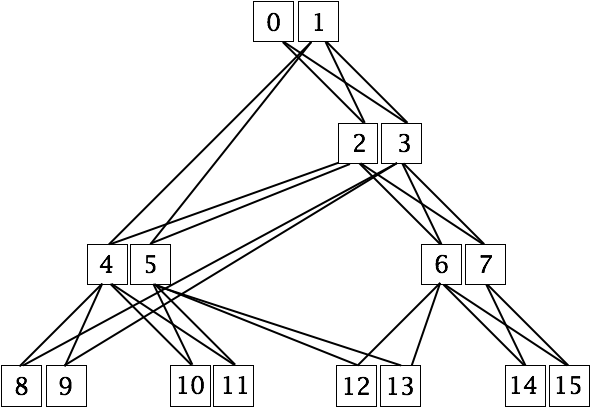
\includegraphics[scale=0.4]{FiguresMaths/FiboFast.png}
        \caption{Dependency relations for computing the pairs $(F(2n),F(2n+1))$.}
                \label{fig:fastFibo}
\end{center}
\end{figure}
In particular, we show how to compute an element ($F(13)$) using the fast Fibonacci scheme in Fig.~\ref{fig:fastFibo13}.
The pattern is embedded into a complete binary tree of predecessors (with some redundancies)
whose depth is logarithmic.
\begin{figure}[h]
\begin{center}
        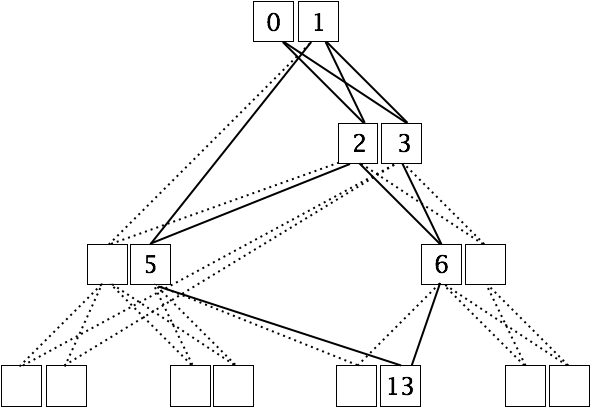
\includegraphics[scale=0.4]{FiguresMaths/FiboFast13.png}
        \caption{Ancestors involved in the computation of $F(13)$. }
        \label{fig:fastFibo13}
\end{center}
\end{figure}
The conclusion is that
any Fibonacci number $F(n)$ can be computed very fast in $log_2 (n)$ steps.



\subsection{Cassini's Identity}

%\noindent \textit{The aim.}
%Prove a classical identity involving Fibonacci numbers, which is a nice example of proof by recurrence.
%\medskip

\noindent \textit{The problem.}
Prove the following expression:

$F(n-1).F(n+1) = F(n)^2 + (-1)^{n+1}$ for $n \geq 1$

where $F(n)$ is the n\textit{th} Fibonacci number.
\medskip

%Let check the expression on the first ranks:
%
%$n=1$, $F(0).F(2) = F(1)^2 +1 = 2$
%
%$n=2$, $F(1).F(3) = F(2)^2 -1 = 3$
%
%$n=3$, $F(2).F(4) = F(3)^2 +1 = 10$
%
%$n=4$, $F(3).F(5) = F(4)^2 -1 = 24$
%
%...
%\medskip

\noindent \textit{The solution.}
The proof is by induction.

The basis case $n=1$ holds since $F(0).F(2) = F(1)^2 +1 = 2$.

The induction step is proved assuming the Cassini's identity holds at rank $n$.
Replace $F(n+2)$ by its definition in the expression:
 
$F(n).F(n+2) = F(n) (F(n+1)+F(n)) = F(n)^2 + F(n).F(n+1)$

Then, replace the last term using the recurrence hypothesis:

$F(n)^2 = F(n-1).F(n+1) - (-1)^{n+1} =F(n-1).F(n+1) + (-1)^{n+2} $

Thus,
$F(n).F(n+2) = F(n).F(n+1) + F(n-1).F(n+1) + (-1)^{n+2} = F(n+1) (F(n) + F(n-1)) + (-1)^{n+2}$ 

Apply again the definition of Fibonacci sequence $F(n) + F(n-1) = F(n+1)$, we obtain:

$F(n).F(n+2) = F(n+1)^2 + (-1)^{n+2}$

This concludes the proof. 


\subsection{Lucas Numbers} 

%\noindent \textit{The aim.}
%Fibonacci progression is the most popular and the most simple Definition of Lucas' numbers
%
\textbf{Definition.}
Given the two starting numbers $L(0) = 1$ and $L(1) = 3$, 
the Lucas numbers are obtained by the same progression as Fibonacci: 

$L(n+1) = L(n)+L(n-1)$.
\medskip

In order to gain intuition on this problem, let us compute the first ranks in regard to the classical Fibonacci numbers:
\begin{figure}[htb]
\[
\begin{array}{c||r|r|r|r|r|r|r|r|r|r|r}
{\displaystyle n } & k=0 & k=1 & k=2 & k=3 & k=4 & k=5 &
k=6 & k=7 & k=8 & k=9 & \ldots \\
\hline
F(n) & 1 & 1 &  2  &  3  &   5  &   8  &  13  &  21  & 34  & 55  & \ldots \\
\hline
L(n) & 1 & 3 &  4 &  7  &  11  &  18  &  29 & 47  & 76  & 123 & \ldots \\
\hline
\end{array}
\] 
\caption{Correspondence between Fibonacci and Lucas numbers.}
\label{fig:fiboLucas}
\end{figure}
%
%n: $~~~~0, 1, 2, 3, ~4, ~5, ~6, ~7, ~8, ~~9, ...$
%
%F(n): $1, 1, 2, 3, ~5, ~8, 13, 21, 34, ~55, ...$
%
%L(n): $1, 3, 4, 7, 11, 18, 29, 47, 76, 123, ...$
\medskip

%
%There are strong links with Fibonacci numbers.
%In particular, we established before that
%\bigskip
%
%$F(n+2) = 1+ \sum_{k=0}^{n} F(k)$. 
%\bigskip
%
%We have similarly: $L(n+2) = 1+ \sum_{k=-1}^{n} L(k)$ since the basic step of the induction is still valid: 
%
%$L(2) = L(-1 )+L(0) +1 = 2+1+1 = 4$.
%%Actually, it will be true for all the progressions where $u_1=1$.
%

\noindent \textit{The problem.}
Prove the following expression:

$F(k-1).L(n) = F(n+k)+ (-1)^{k-1}F(n-k)$ for $k \leq n$
\bigskip

\noindent \textit{The solution.} 

There are two integers involved here ($k$ and $n$).
Let us study the expression step by step for successive values of $k$.
\medskip

\begin{itemize}
\item Starting smoothly with $k=1$

We can easily show by induction on $n$ that the Lucas number of order $n$ is the sum of two Fibonacci numbers:

$L(n) = F(n-1)+F(n+1)$ for $n \geq 1$
\medskip

%Let check this property on the first ranks:
%
%$n=2$, $L(2) = F(1)+F(3) = 1 + 3 = 4$
%
%$n=3$, $L(3) = F(2)+F(4) = 2 + 5 = 7$
%
%$n=4$, $L(4) = F(3)+F(5) = 3 + 8 = 11$
%
%$n=5$, $L(5) = F(4)+F(6) = 5 + 13 = 18$
%

The basis case, corresponding to for $n=1$) is true since $L(1) = 3 = F(2) + F(0) = 2+1$.

Let assume for proving the induction step that the property holds at all ranks $k \leq n$ and compute $L(n+1)$:

Apply the definition of Lucas' numbers: $L(n+1) = L(n)+L(n-1)$

Apply the induction hypothesis on both terms of the right hand side:

 $L(n+1) = F(n+1)+F(n-1)+F(n)+F(n-2)$

Apply now the definition of Fibonacci numbers for $F(n+1) + F(n) = F(n+2)$  and $F(n-1) + F(n-2) = F(n)$

Replace them in the previous expression:

$L(n+1) = F(n+2)+F(n)$

which concludes the proof.

\item
Extension.

Using a similar approach, we obtain $L(n) = F(n+2)-F(n-2)$. 
What happens if we generalize? 
\medskip

Easy calculations lead to the following results:
\medskip

$2.L(n) = F(n+3) + F(n-3) $

%Proposition.
%
%$2.L(n) = F(n+3)+F(n-3)$
%\bigskip
%
%Proof.
%We start from $L(n) = F(n+2)-F(n-2)$
%
%$F(n+2) = F(n+3) - F(n+1)$ and $F(n-2) = F(n-1) - F(n-3)$
%
%$L(n) = F(n+3) - (F(n+1) + F(n-1)) + F(n-3)$
%
%$2.L(n) = F(n+3) + F(n-3)$
%
%
%\item Extension 2
%
%Go to the next step using the same technique:
%\medskip
%
%
%
%$= F(n+4) - F(n+2) + F(n-2) - F(n-4)$
%\medskip

$3.L(n) = F(n+4) - F(n-4)$

$5.L(n) = F(n+5) + F(n-5)$
\medskip
 
As $2, 3, 5$ are successive Fibonacci numbers, this gives us the intuition of the general case:

$F(k-1).L(n) = F(n+k) + (-1)^{k-1}F(n-k)$ for $k \leq n$
\medskip

which is proved (again) as follows by induction assuming the expression holds at rank up to $k$.

The basis case is straightforward (see case $k=1$).

Compute $F((k+1)-1).L(n)$ and apply the definition of Fibonacci number $F((k+1)-1) = F(k-1) + F(k-2)$

$F(k).L(n) = F(k-1).L(n + F(k-2).L(n)$ and replace both last terms by using the induction hypothesis:

$= F(n+k) + (-1)^{k-1}F(n-k) + F(n+k-1) + (-1)^{k-2}F(n-(k-1))$

$= F(n+k) +  F(n+k-1) + (-1)^{k-1}(F(n-k) - F(n-k+1))$

The final result is obtained by applying twice the definition of the Fibonacci numbers.
%\medskip
%
%\noindent \textit{Lesson learned.}
%This exercice is a good example of the proof of a non straightforward recurrence which involves two integers.

\end{itemize}

\subsection{Solving a bilinear recurrence by a linear system}

\noindent \textit{The problem.}
The goal here is to determine the values of  $U_n$

Solve $U_{n} = \frac{1}{2}.U_{n-1} + \frac{1}{2}.U_{n+1}$

knowing $U_0 = 0$ and $U_N = 1$
\medskip

\noindent \textit{The solution.}




\ignore{
*****\subsection{Lucas' numbers}

\noindent \textit{The problem.}

Prove the following expression.
 
$F(n+1) = \frac{1}{2} (F(0).L(n) + F(n).L(0))$
\medskip

\noindent \textit{The solution.}
The proof comes from direct arithmetic manipulations:

$2.F(n+1) = F(n+1) +  F(n+1) =  F(n+1) + F(n) + F(n-1)$

$= L(n) + F(n) $

$= F(0).L(n) + F(n).L(0)$
\medskip

\noindent \textit{The problem.}

The previous property can be extended for any $m>1$ as follows:
\medskip

$2.F(n+m) = F(m-1).L(n) + F(n).L(m-1)$
\medskip

\noindent \textit{The solution.}
The proof is by recurrence on $m$ considering any fixed $n$.
\begin{itemize}
\item
The \textbf{basis case} (for $m=1$) is given by the previous proposition.

\item
\textbf{Induction step:} 
Assume the property holds at rank $m > 1$ and consider $F(n+m+1)$:

Apply the definition of Fibonacci numbers: 

$F(n+m+1) = F(n+m)+F(n+m-1)$ 

Replace both terms by the recurrence hypothesis:

$= \frac{1}{2} (F(m-1).L(n) + F(n).L(m-1)) + \frac{1}{2} (F(m-2).L(n) + F(n).L(m-2))$

$= \frac{1}{2} \left( (F(m-1)+F(m-2)).L(n) + F(n).(L(m-1)+L(m-2))\right)$

$= \frac{1}{2} \left(F(m).L(n) + F(n).(L(m)\right)$
\end{itemize}
***** }

%%%%%%%%%%%%%%%%%%%%%%%%%%%%%%%%%%%%%%%%%

\section{Chapter 10}

\subsection{Application of the Fundamental Theorem of Arithmetic}
%
%\noindent \textit{The aim.}
%Significant application of the Fundamental Theorem of Arithmetic~\ref{thm:Fund-Thm-Arith}.
%\medskip

\noindent \textit{The problem.}
For all $\langle x,y \rangle \in \N^+ \times \N^+$

$\a(x,y) \ \eqdef \ 2^{x-1} \cdot (2y -1)$

verify function $\a$'s bijectiveness.
\medskip

\noindent \textit{The solution.}

\medskip
%
%\noindent \textit{Lesson learned.}



\subsection{The average length of a carry in a binary counter}

\noindent {\it The problem.}
%
You add from $1$ to $n$, in increments of $1$ using a counter of
binary (or, base-$2$) numerals.  Each time you increment the counter,
there is a {\it carry}.  These carries have varying lengths; for
instance, when $n = 32 = 100000_2$, the carry-lengths range
from $0$---whenever you increment an even integer---to $5$---when you
increment $31 = 11111_2$ to achieve $32 = 100000_2$. \\
{\em Prove that the average carry as you go from $1$ to $n$ has length $2$.}
\medskip

\noindent {\it The solution.}

\noindent
Half of the increments add $1$ to an even number, i.e., a number whose
binary numeral ends in ``$ \ldots 0$''.  These increments generate no
carry---or, equivalently, a carry of length $0$.

\noindent
One-quarter of the increments, which form half of the remaining
increments, execute a carry of length $1$, because they add $1$ to a
numeral that ends in ``$ \ldots 01$''.

\noindent
One-eighth of the increments, which form half of the remaining
increments, execute a carry of length $2$, because they add $1$ to a
numeral that ends in ``$ \ldots 011$''.

Continuing in this way, one can show that the average length of a
carry can be expressed in the form
\[ 
\frac{1}{2} \cdot 0 \ + \ \frac{1}{4} \cdot 1 \ + \ \frac{1}{8} \cdot
3 \ + \ \frac{1}{16} \cdot 4 \ + \ \cdots
\]
Using techniques that we cover in Chapter~\ref{ch:Summation}, one
verifies that this infinite series converges with the sum $2$.  \qed




%%%%%%%%%%%%%%%%%%%%%%%%%%%%%%%%%%%%%%%%%

\section{Chapter 11}

\subsection{Going further in a game analysis}

\noindent \textit{The problem.}
Analyze the game of craps in the same way as we did for sum-of-three

Verify the table in Fig.~\ref{fig:dice-ordered-configs}

In the ordered version of sum-of-three, sum$k$ is engendered by the
same number of configurations as is sum $21 - k$.  
Why is this the case?

\noindent \textit{The solution.}


\subsection{more about the Birthday paradox}

%\noindent \textit{The aim.}
%An interesting variant of the birthday puzzle
%\medskip
%
%\noindent \textit{The problem.}
Determine the
probability of a student to be born the same day as me.
\medskip

\noindent \textit{The solution.}



\subsection{A property about binomial coefficients}
%
%\noindent \textit{The aim.}
%xx
%\medskip

\noindent \textit{The problem.}
Prove the following property by two ways (recurrence and by using a combinatorial argument

$\forall n,k$ $1 \leq k \leq n$

$k.{n \choose k} = n.{{n-1} \choose {k-1}}$
\medskip

\noindent \textit{The solution.}




%%%%%%%%%%%%%%%%%%%%%%%%%%%%%%%%%%%

\section{Chapters 12}


\subsection{Formal definition of mesh graphs}
\label{Exercice:FormalDefinitionMesh}
%
%\noindent \textit{The aim.}
%The definition of mesh presented in chapter~\ref{ch:Graphs1}
%is very easy to capture with a drawing.
%We formalize here the precise definition using a mathematical language. 
%\medskip

\noindent \textit{The problem.}
Formalize precisely the definition of mesh  $\m_{m,n}$ and torus $\widetilde{\m}_{m,n}$ graphs
for positive integers $m, n \in \N^+$.
\medskip

\noindent \textit{The solution.}
The  {\it vertex-set} is the same for both graphs:

\begin{eqnarray*}
\n_{\fm_{m,n}} \ = \ \n_{\widetilde{\fm}_{m,n}}
  & = & 
\{1, \ 2, \ldots, \ m\} \ \times \ \{1, \ 2, \ldots, \ n\} \\
  & = & 
\big\{ \langle i, \ j \rangle \ \ | \ \ 
\big[ i \in \{1, \ 2, \ldots, \ m\} \big], \ \
\big[ j \in \{1, \ 2, \ldots, \ n\} \big]
\big\}
\end{eqnarray*}


$\m_{m,n}$ has $(m-1)n \ + \ (n-1)m$ edges; its {\it edge-set} is
\begin{eqnarray*}
\e_{\fm_{m,n}} & = & 
\big\{
\{ \{ i, j \}, \ \{ i+1, j \} \ \ | \ \
1 \leq i < m, \ \ 1 \leq j \leq n \} \\
  &  & \hspace*{.1in} \cup
\{ \{ i, j \}, \ \{ i, j+1 \} \ \ | \ \
1 \leq i \leq m, \ \ 1 \leq j < n \}
\big\}
\end{eqnarray*}

\medskip

The subgraph of $\m_{m,n}$ defined by the vertex-set
\[ \{ \langle i, \ j \rangle  \ \ | \ \ \left[i \in \{1, 2, \ldots,
  m\}\right], \ \ \left[1 \leq j < n\right]\}
\]
and all edges both of whose endpoints belong to that set is called the
$i$th {\it row} of $\m_{m,n}$
Dually, the subgraph of $\m_{m,n}$ defined by the vertex-set
\[ \{ \langle i, \ j \rangle  \ \ | \ \ \left[j \in \{1, 2, \ldots,
  n\}\right], \ \ \left[1 \leq i < m\right] \}
\]
and all edges both of whose endpoints belong to that set is called the
$j$th {\it column} of $\m_{m,n}$.


\begin{itemize}
     \item
Vertices $\langle 1, \ 1 \rangle$, $\langle 1, \ n \rangle$, $\langle m,
\ 1 \rangle$, and $\langle m, \ n \rangle$ are the {\it corner vertices}
(or, just {\it corners}) of $\m_{m,n}$.
     \item
The path-graph consisting of the vertex-set
\[ \{ \langle 1, \ 1 \rangle, \ \langle 1, \ 2 \rangle, \ldots, \
\langle 1, \ n \rangle \}
\]
together with all edges of $\m_{m,n}$ both of whose endpoints belong
to this set, is the {\it top edge} of $\m_{m,n}$.

The other edges of $\m_n$ are defined analogously:

\medskip

The {\it bottom edge} of $\m_{m,n}$ is the path-graph built upon the
vertex-set
\[ \{ \langle m, \ 1 \rangle, \ \langle m, \ 2 \rangle, \ldots, \
\langle m, \ n \rangle \}
\]

The {\it left edge} of $\m_{m,n}$ is the path-graph built upon the
vertex-set
\[ \{ \langle 1, \ 1 \rangle, \ \langle 2, \ 1 \rangle, \ldots, \
\langle m, \ 1 \rangle \}
\]

The {\it right edge} of $\m_{m,n}$ is the path-graph built upon the
vertex-set
\[ \{ \langle 1, \ n \rangle, \ \langle 2, \ n \rangle, \ldots, \
\langle m, \ n \rangle \}
\]
\end{itemize}
\medskip

Same for the torus graphs:

The subgraph of $\widetilde{\m}_{m,n}$ defined by the vertex-set
\[ \{ \langle i, \ j \rangle  \ \ | \ \ \left[i \in \{1, 2, \ldots,
  m\}\right], \ \ \left[1 \leq j \leq n\right]\}
\]
and all edges both of whose endpoints belong to that set is called the
$i$th {\it row} of $\widetilde{\m}_{m,n}$
Dually, the subgraph of$\widetilde{\m}_{m,n}$ defined by the vertex-set
\[ \{ \langle i, \ j \rangle  \ \ | \ \ \left[j \in \{1, 2, \ldots,
  n\}\right], \ \ \left[1 \leq i \leq m\right] \}
\]
and all edges both of whose endpoints belong to that set is called the
$j$th {\it column} of $\widetilde{\m}_{m,n}$.
%\medskip
%
%\noindent \textit{Lesson learned.}
%manipulate mathematical symbols. 


%%%
\subsection{Graph Isomorphism}

\noindent \textit{The problem.}
The order-$4$ hypercube $\q_4$ is \textit{isomorphic} to the $4 \times
4$ torus $\widetilde{\m}_{4,4}$.
\medskip

\noindent \textit{The solution.}
We describe both coding schemes successively. 

$\q_4$ is represented by its natural Gray codes,
where a vertex is coded 4 bits and connected to its four neighbors by complementing 
the digit in each of the four dimensions.
\medskip

$\widetilde{\m}_{4,4}$ is the cartesian product between two mono-dimensional rings.
Each one is composed of the four vertices connected using a Gray code:

$00, 01, 11, 10$

The whole coding is obtained by concatenation of both dimensions.


%%%%%%%%%%%%%%%%%%%%%%%%%%%%%%%%%%%%%%%%
\section{Chapters 13}


\subsection{Euler Formula}

\noindent \textit{The aim.}
Complete a result of the termination with a connected tree.
\medskip

\noindent \textit{The problem.}
Prove the termination with a connected tree should be an
  exercise.
  
Phase 1 of the proof by deconstruction of Euler's formula
\medskip


%%%
\subsection{Proving a negative result}

\noindent \textit{The aim.}
Show the proof of a negative result.
\medskip

\noindent \textit{The problem.}
Show that the graph $K_{3,2}$ is not outerplanar.
\begin{figure}[h]
\begin{center}
        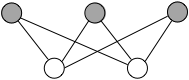
\includegraphics[scale=0.4]{FiguresGraph/outerplanarK3,2init}
        \caption{$K_{3,2}$ with its two types of vertices that are not connected two by two (white and shaded).}
\end{center}
\end{figure}
\medskip

\noindent \textit{The solution.}

We recall that a graph is outerplanar if there exists a representation where its vertices are distributed along a circle 
and no edges are crossing each other.

The solution is a case by case analysis according to all the possibilities to distribute the vertices on a circle.
\begin{figure}[h]
\begin{center}
        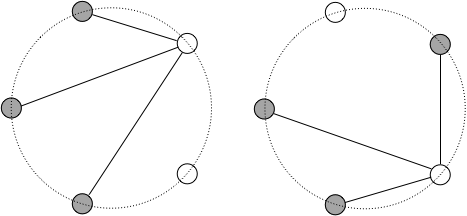
\includegraphics[scale=0.4]{FiguresGraph/outerplanarK3,2}
        \caption{The two possibilities to distribute the white and shaded vertices along a circle.}
\end{center}
\end{figure}

\medskip

\noindent \textit{Lesson learned.}


%%%
\subsection{Outerplanar graphs}

\noindent \textit{The aim.}

\medskip

\noindent \textit{The problem.}
Show that every outerplanar graph is a subgraph of a Hamiltonian graph.
\medskip

\noindent \textit{The solution.}

\medskip

\noindent \textit{Lesson learned.}


%
%%%%
%\subsection{Spanning Trees}
%\label{Exercice:spanningTrees}
%
%{\Denis I don't think it is mandatory to have such an exercice, the objective is not clear for me
%and it is too complicated -- and more algorithms than Maths...}
%
%Recall here the problem
%\medskip
%
%There are mainly two ways for constructing such a MST, each one
%emphasizes a different propriety of the MST, namely, avoid cycles and
%minimize the span.  In both cases, the edges are sorted in increasing
%order of weights.  More precisely, the first one constructs a subtree
%which partially spans the graph by adding at each step the minimum
%neighboring edge while the other add successively the edges of minimal
%weights that do not create a cycle.




